\label{sec:sokar-gui}

\par
Po uruchomieniu programu użytkownikowi ukazuje się głowne okno, pokazane na rysuneku \ref{fig:sokar-gui-empty-window}, implemntowane przez klasę \sokarclass{MainWindow}.
Okno zawiera 3 elementy: menu (obiekt klasy \qtclass{QMenuBar}), drzewa plików (obiekt klasy \sokarclass{FileTree}), obiekt zakładek z obrazami (obiekt klasy \sokarclass{DicomTabs}).

\begin{figure}[!htbp]
    \centering
    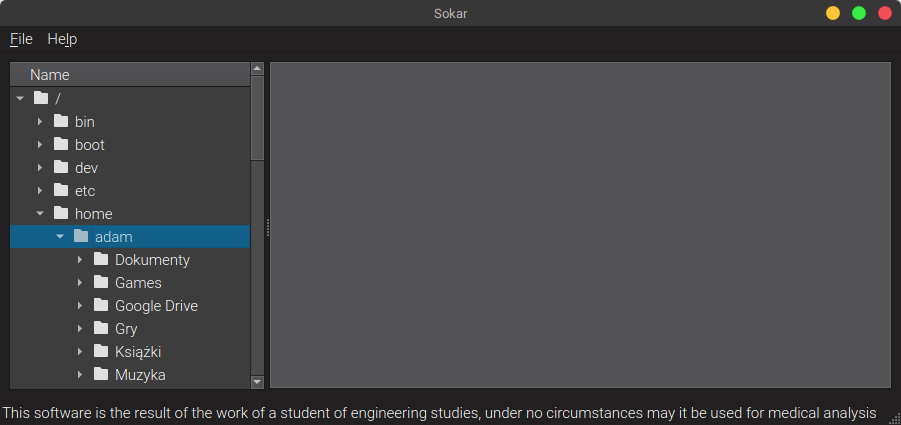
\includegraphics[width=0.7\textwidth]{img/sokar-gui-001.png}
    \caption{Okno przeglądarki tuż po uruchomieniu. Zdjęcie własne.}
    \label{fig:sokar-gui-empty-window}
\end{figure}

\par
Użytkownik może otworzyć plik \DICOM na trzy sposoby: z menu na górze, z drzewa ze strukturą pików i poprzez przeciągnięcie.
W dwóch pierwszych przypadka użytkownik może otworzyć tylko jeden plik na raz, ale w trzecim jest możliwość wczytania wielu plików.

\par
Po wczytaniu, pliki są wyświetlane w zakładach.
Kontener z zakładkami jest implementowanych przez klasę \sokarclass{DicomTabs}.
Przykład programu z wczytanymi kilkoma plikami, w tym jednym z animacja znajduje się na rysunku \ref{fig:sokar-gui-with-files}

\begin{figure}[!htbp]
    \centering
    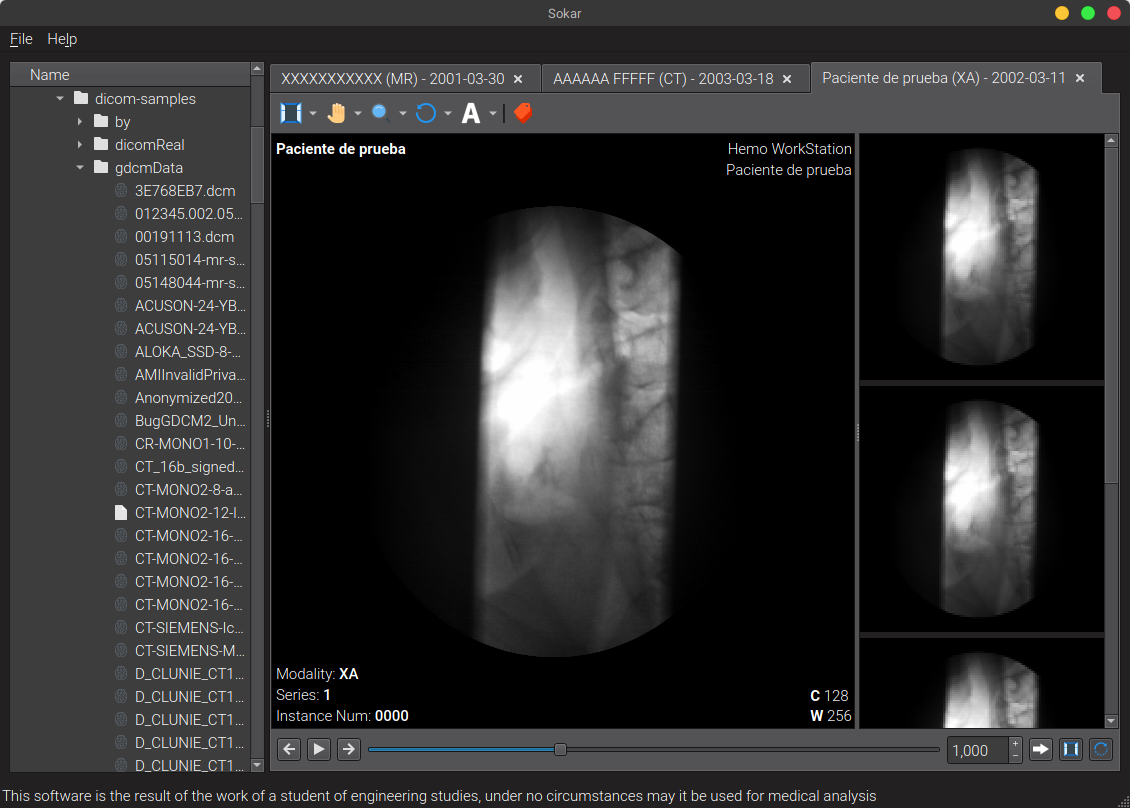
\includegraphics[width=\textwidth]{img/sokar-gui-002.png}
    \caption{Okno przeglądarki z wczytanymi kilkoma obrazami. Zdjęcie własne.}
    \label{fig:sokar-gui-with-files}
\end{figure}

\par
Obiekt wewnątrz zakładek odpowiada za wyświetlanie wszystkich elementów umożliwiających interakcje użytkownika z obrazem, jest implementowany przez klasę \sokarclass{DicomView}.
Jeden taki obiekt może posiadać wiele obrazów wyświetlanych w formie animacji.
Obrazy są wyświetlane na scenie implementowanej przez \sokarclass{DicomScene}.
Pod sceną znajduje się pasek filmu, za pomocą, którego użytkownik może zatrzymać lub wznowić animację.
Na prawo od sceny znajdują sie ikony i wszystkimi ramkami filmu.
Pasek filmu i ikony obrazów ukrywają się gdy jest wczytany tylko jeden obraz.
\par
Scena to obiekt wyświetlający i generujący obraz na ekranie.
Dodatkowo na scenie jest znajdują się pięć zestawów informacji z pliku \DICOM.
Dane pacjenta w lewym górnym rogu.
Danych szpitala lub jednostki w której obraz został wykonany w prawym górnym rogu.
Danych akwizycji obrazów w lewym dolnym rogu, mogących sie różnić dla każdej modalności.
Podziałka informująca o rzeczywistym rozmiarze obiektu znajdującego się na obrazie znajdująca się w dolnej i prawej części obrazu.
Cztery litery z sześciu (H, F, A, P, R, L) informujących o ułożeniu obrazu względem pacjenta.
Przykładowa scena z obrazem monochromatycznym znajduje sie na rysunku \ref{fig:sokar-gui-scene}.

\begin{figure}[!htbp]
    \centering
    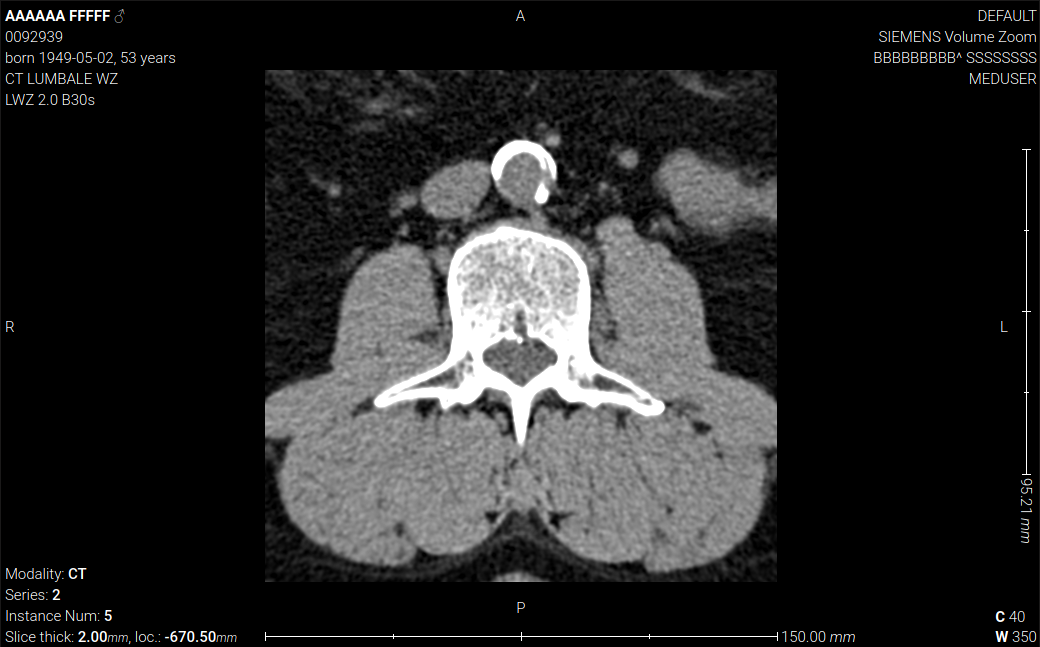
\includegraphics[width=\textwidth]{img/sokar-gui-003.png}
    \caption{Przykładowa scena z obrazem monochromatycznym. Zdjęcie własne.}
    \label{fig:sokar-gui-scene}
\end{figure}

\par
Możliwość wyświetlania animacji pojawia się wtedy gdy w jeden zakładce będzie znajdowało się więcej niż jedna ramka obrazu.
Można to osiągnąć wczytując wiele obrazów z tej samej serii lub wczytać obraz posiadający wiele ramek.
Wówczas pod sceną pojawia się pasek, umożliwiający sterowanie animacją, a po prawej stronie obiekt z ikonami poszczególnych ramek obrazu.
Dokładny opis przycisków i ich funkcji znajduje się w sekcji .


\par
Struktura menu programu znajdującego się na górze:
\begin{itemize}
    \item File
          \begin{itemize}
              \item Open --- otwiera okienko wyboru plików
              \item Open Recent --- lista z ostatnio otworzonymi plikami
              \item Export as --- zapisanie obrazu w formacie JPEG, BMP, GIF lub PNG.
              \item Exit --- wyjście z aplikacji
          \end{itemize}
    \item Help
          \begin{itemize}
              \item About Qt --- otwiera okno informacji o bibliotece Qt.
              \item About GDCM --- otwiera okno z informacjami o bibliotece GDCM
              \item About Sokar --- otwiera okno z informacjami o aplikacji
          \end{itemize}
\end{itemize}